\documentclass[10pt]{article}
\usepackage{fullpage}
\usepackage{flafter}
\usepackage{hyperref}
\usepackage{graphicx}
\begin{document}
\title{\underline{ARM - Report}}
\author{Gauthier Bonvarlet, Theo Cohen, Sebastian Kovats, Marco Violet-Vianello}
\maketitle
\section{\underline{Project structure}}
\bigskip

The structure of the project is as follows:
\begin{itemize}
\item src/assembler contains all the source files of the assembler
\item src/emulator contains all the source files of the emulator
\item src/led contains the assembly file that activates GPIO 16 of the Raspberry Pi.
\item HaikuBerry/ contains the source files of our extension
\end{itemize}

\section{\underline{Emulator and Assembler}}
\bigskip

We kept our assembler and emulator as independent programs. Their designs are as follows:

\subsection{\underline{Emulator}}
\bigskip

\begin{itemize}
\item \textbf{main.c}: The entry point of the program handles the parsing of the program arguments and reading the binary file as an array of 32-bit data chunks. The chunks are then processed in the main pipeline loop, which delegates to executor.c
\item \textbf{executor.c}: Here the execute function checks for the type of instruction and whether it is valid according to the condition bits. It then delegates to the relevant functions for data processing, multiplication, branching and data transfer.
\item \textbf{data\_processing.c}: Since data processing is actually many different instructions we decided to put these functions in a separate file.
\item \textbf{utils.c}: This file contains various utility functions that are used across the program, such as for setting specific flags in the CPSR register or printing the state of the registers and memory.
\item \textbf{typedefs.h}: Here we define various data types for use in the program and model the state of the machine as the struct Registers, which is passed to all functions that manipulate it.
\item \textbf{tests.c}: We used this file to place debugging functions which print information about a given instruction, such as its type and source/destination registers. This turned out to be invaluable in later stages of development.
\end{itemize}

\subsection{\underline{Assembler}}
\bigskip

\begin{itemize}
\item \textbf{main.c}: After parsing the program arguments the main function allocates the output binary array and calls generate\_symboltable. It then enters the main loop, which for each assembly instruction first extracts the semantic information contained in an instruction into a Token struct, which is then used by generate\_bit\_instructions to make the corresponding bit pattern.
\item \textbf{symboltable.c/h}: These files contain generate\_symboltable and lookup\_symboltable, as well as some typedefs and helper functions.
\item \textbf{parser.c}: The main function here is parse\_instr, which handles the extraction of all semantic information from an assembly line into a Token struct by delegating to various auxiliary functions whose responsibilities follow the syntactic structure of assembly instructions. It also contains some more general string manipulation helper functions.
\item \textbf{typedefs.h}: Here we defined our custom data types used across the program. The most complex one is Token, which encodes all information contained in an instruction in a directly accessible format, used by the assembler to easily create the corresponding bitpattern from it.
\item \textbf{assemble.c}: Given the information stored in a Token struct, create\_instr\_bits delegates to helper functions for specific instruction types to create a finished binary instruction.
\item \textbf{utils.c}: The file contains two helper functions used by main, read\_text, which reads a text file into a char array and print\_hex, which prints the hexadecimal representation of a number as it is laid out in a little-endian system.

\end{itemize}

\subsection{\underline{Testing}}
One of the vital tools we had to test our implementation was the Ruby test-suite. We managed to set this up during the first week of the project. We believe the test suite was very useful as it gave us a global idea of how well our emulator and assembler were working. After running the test-suite we knew which categories of instructions were failing and but it also provided a few edges cases. However, this test suite did not provide us enough information as to where our program was failing. Furthermore running it after every single modification was a bit time consuming and not really efficient. So most of the time, we would run our program locally and pass as an argument a single file path. Indeed we designed two different modes for testing, one for the test-suite and one for running our program locally with a single file path. One of the main tools we have used is the CLion debugger in conjunction with gdb. One of the advantages of using gdb is printing variables in a certain format such as hexadecimal at a precise memory location. This was very useful since we were dealing with binary representation. However, the Clion debugger has a better interface. A combination of both meant we were quite efficient in debugging. Furthermore, another idea we had for testing was the use of custom made tokens. Indeed for the assembler part, we had to put a lot of work into parsing the assembly instructions to generate tokens but we also needed to build in parallel the functions that would produce the binaries. So we built custom made tokens which we would pass onto our different functions to test them while the parsing was being built. Another tool we used is Valgrind. We felt is was particularly usefull to detect and fix memory leaks and it generally provided valueble insights into out programs. We feel a good balance between running the test-suite and running our program locally was key to debugging effciently.

\section{\underline{GPIO}}
For part III, we first installed Raspbian on the Pi. Then, we wrote the ARM program which sets the pin 16th as an output, then iteratively sets off and on this pin, in an endless loop. We had to add a very long loop between each setting on/off in order to make a pause between changes. Then, when ran \textit{make} which also assembles the ARM program creating a binary file \textit{kernel.img}. Finally, we replaced the kernel of the pi by this one which had the consequence to make the LED (gpio 16) blink.
\begin{figure}[h!]
\centering
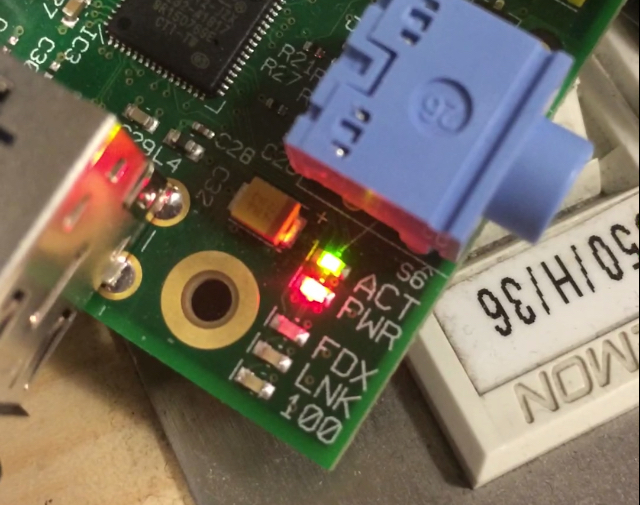
\includegraphics[width=10cm]{IMG_B28F30CC1D47-1}
\caption{Gpio 16/LED blinking}
\end{figure}
\bigskip
\bigskip

\section{\underline{Extension - HaikuBerry}}

\subsection{\underline{Description}}
Our extension is \textit{HaikuBerry}, a generator of Haiku poems which delivers it with a voice synthesis system. Given a database of words and grammar syntaxes, it randomly assembles a Haiku and uses a speech library to read it out loud.
\paragraph{The Haiku}\mbox{}\\
A Haiku is a traditional Japanese poetic form which consists of three lines (stanzas) of 5, 7 and 5 syllables respectively.
\paragraph{Databases}\mbox{}\\
Our generator uses two databases (.txt files). The first one is a dictionary which is a list of words along with information about their type and syllable count, like:
\begin{center}
\textless word type\textgreater,\textless number of syllables\textgreater,\textless
word\textgreater
\mbox{}\\
e.g. noun,1,duck stands for the onesyllabic word duck
\end{center}
A Word type can be a noun, adjective, adverb, verb (transitive or intransitive) or determinant. The database we used contains words of up to 4 syllables but the design of the parser allows for an arbitrary syllable count.\newline
The other database is a list of possible formats of the haiku i.e. the grammar construction of the poem with some pre-written parts. For example, given the following structure, our program produced the output:\newline\newline
\leavevmode\hbox to \linewidth{%
\begin{tabular}[t]{l@{}}
     @  \\
     I was in that, noun 1, \$NL, \\
     deter 1, noun 1, was, adj 1, and, adj 2, \$NL, \\
     I, verbi 1, adverb 3 \\
\end{tabular}
\hfill
\begin{tabular}[t]{l@{}}
	\\
    I was in that lust, \\
	His ice was fresh and sunny, \\
	I thought carefully \\
\end{tabular}%
}
\mbox{}\\
\mbox{}\\
Then, the program parses all of this data into two data structures Dictionary and Haiku. Dictionary holds, for each type of words, an array of words arrays with a specific number of syllables. Hence, there is an array for nouns of 1 syllable, 2 syllables, adjectives of 1 syllable and so on.
The other structure, Haiku, holds an array of all the possible haiku formats.
Once it has parsed all the data, the program picks randomly a haiku format and then fills the word gaps (randomly again) with an appropriate word type and syllables count. The string created is written in a text file.\newline 
Finally, the program launches a terminal command to make the text file read by the speech synthesis library \href{http://www.cstr.ed.ac.uk/projects/festival/}{\textit{Festival}}.
\paragraph{The Product}\mbox{}\\
So far, the program is running on the Raspberry Pi connected to a speaker and a button which when pressed, creates a new Haiku and reads it out loud.\newline
The goal for the presentation is to make a final product on the Pi which run in headless power mode, that is to say that the program would run automatically at the start-up of the pi without the need to set it up with a display.\newline

\subsection{\underline{Reflection}}
It took us some time to find an idea that satisfied us. Indeed, we wanted to do something artistic because we wouldn't have created something truly useful in this amount of time. We also wanted to use mostly C and not depend on pre-made libraries, as well as to implement at least one input and one output on the raspberry pi. The Haiku idea suited these requirements perfectly.\newline
Our first idea was to generate haikus by recursively generating lines of a given number of syllables completely randomly, e.g. we had a function to generate 5 syllables that would then randomly decide whether to pick a word with 5 syllables, pick two with two syllables and one with one,... However, this approach soon turned out to produce nothing meaningful, so we decided to introduce a type tag in the word library and define gramatically meaningful poems of the required length and rhythm ourselves. This implementation also allows for more freedom to define other types of poems of arbitrary length and rhythm.
One challenging part of the work was, as in the assembler, dealing with the efficient extraction of information from a text file. Memory leaks also turned out to be tricky to fix but we managed thanks to Valgrind. In general our testing was similar to the assembler and emulator where we made extensive use of gdb and the CLion debugger to gain an insight into how our program works. \newline

\section{\underline{Group reflection}}
Overall, our group organisation was quite good during the entirety of the project. We would usually discuss the general design of the solution we wanted to implement in order to make sure each team member was on the same page and knew what they were doing. Once we had come to an agreement, usually one or two of us would start building the foundations that we would need such as structs, testing environment and debug mode. We could then work on our parts independently. Splitting the parts worked well, even though some group members went faster than others due to the varying difficulty of the tasks. This was not an issue since we would work in group on the harder problems to be more efficient. We never came to a point when we thought we had nothing to do because every team member was very proactive. This work ethic was efficient and we will try to maintain it in future group project. Communication would happen in two different ways, either online or face to face. We preferred meeting each other regularly to work altogether but most importantly to discuss complex concepts and solutions. Another indirect way of communicating was reading commit messages and regularly checking the version control graph. This gave us a overall view of the projects progress of specific parts each of us were working on. From this, we would give ourselves feedback regularly and this helped us improved our style and readability. Again, we thought this was a positive way of progressing and keeping up to date with the project's structure. On many occasions, we rewrote code that we had already written to make sure the final product was the best version possible.

\subsection*{\underline{Marco}}
During this group project, I had the opportunity to apply what we have learned in our C lectures and work as a team to solve fairly large and complex problems. I believe the group dynamic was great and that we managed to each use our skill-set to the benefit of the group and learn from each other in the process. I personally really enjoyed our discussions on how to solve problems as I could see different approaches that I had not considered which allowed me to improve my problem-solving skills. Moreover, I thought this project was a great opportunity to master 'Git' and understand how to work with others on a same project. Nevertheless, some issues along the way were tricky to solve and we often programmed and debugged in groups of 2, 3 or even the four of us. I thought this made us particularly efficient because some concepts were difficult to conceive on our own, therefore, as a team we managed to make sure that no details were left out.

\hspace*{0.6cm}Additionally, this project has taught me to be more rigorous and consistent in my code as I would constantly strive to make sure that the code I passed on to my co-workers was the best possible and easy to work with. This was achieved through concise and accurate commenting as well as a clean and (as much as possible) elegant code. Overall, thinking back, this project has also sparked my interest to learn more about Ruby, as I had a look through the code for running the test suite to understand how it worked, and about the Raspberry Pi where I had never been able to have a hands-on experience. As a result of this I bought one as well as kit (LEDs, sensor, etc) and spent time learning on my own so that I could bring my new skills and experience to the benefit of the group in the extension.\newline

\subsection*{\underline{Gauthier}}
I believe I fitted well into the group. I managed to work independently on different parts of the code while offering help to my group mates. I enjoyed doing pair-programming with Sebastian, Marco and Theo. I believe we benefited from having small sessions of those. This meant we were more efficient, since we detected bugs earlier and discussed different point of views in implementation. I believe one of the strengths I have developed during the project is debugging. I feel I now approach debugging in a more logical and pragmatic way. On of the weaknesses I believe I had before starting the project was writing code in a concise way. By inspecting, my group's code, I have gained in experience and I believe my style has improved a great deal. I am now constantly looking to find an efficient and elegant solution to a given problem, while preserving readability.  

\hspace*{0.6cm}I also feel I contributed to the overall design of solutions which was made possible by the way we worked as a group. A really positive point for our group was constantly keeping track of the progress of others. As a result we progressed as a 4 and everybody had a good knowledge of every components which made up our entire solution. As a Joint Maths and Computing student, I am happy to have done this project because I got to understand more about Computer architecture and C language which provides a firm understanding of low level operations and memory. I am also happy to have done this group project as it has provided me with valuable team working skills such as coordination which is something we need to acquire before working in industry. Working in a group was challenging but very rewarding.

\subsection*{\underline{Theo}}
My first experience of group programming was very insightful since I discovered difficulties that arise when working in a group, but I also appreciated group benefits.\newline
On one hand, I witnessed the usual challenges that we face in a project such as planning and splitting the work, sharing common bits of code or staying synchronised with git. For me, the trickiest aspect I faced in the group project was to define clearly what I had to do and then be able to use code previously made by others while making mine clear enough for them.\newline
\hspace*{0.6cm}On the other hand, I enjoyed the synergy of a group, as we could see the project progressing at a fast pace and it was satisfying to see that individual contributions put together resulted something consequent. Also, I appreciated the available help of my group mates when needed. Pair programming was another positive discovery for me as I benefited of complementary skills which was enlightening. Hence, I think it made me progress a lot to work with others and it was interesting to see different methods and approaches to a problem. As for communication, I think we were all well aware of the current progress which made things go smoothly.\newline 
\hspace*{0.6cm}As for myself, I think I fitted well in this group of friends where I have learnt to work with. I enjoyed solving problems with them and I think we all built on our ability to work in group and to communicate. Overall, I have been able to work on my group working weaknesses and I have now a clear view on how to approach group programming.  


\subsection*{\underline{Sebastian}}
Admittedly the project required a much more extensive set of skills than just the kind of programming we were used to from our weekly tutorials. The fact that we had no prior exposure to C and no skeleton or guidance on the implementation, in addition to having to coordinate our work with each other, meant that the usual way of just following the spec's suggested implementation was obsolete. As such, I think we rushed a bit to produce code when we started with the emulator, without having fully defined the structure and identified the specific tasks that were needed to split the work efficiently. After this I took up much of the high-level planning for the rest of the project so we could progress efficiently. It was quite demanding to keep the whole picture in mind and set out program designs in advance but I think this is essential in a group project. Thus when we started on the assembler it took us a day to come up with its structure but it was well worth it as we could then work more independently and efficiently. \newline
\hspace*{0.6cm}Throughout the project I pushed a lot for good coding style (comments, modularity, isolation…) which was sometimes met with resentment but I believe is essential in any programming project, especially when others need to work with one’s code. My debugging skills also greatly benefitted the group and I was happy to teach them to the rest of the team, who could thus improve their productivity.
Overall I really enjoyed the project, as I feel it pushed me to outgrow myself and looking back I am proud of what we managed to create. In hindsight I believe we would have been more efficient had we assigned the assembler and emulator to teams of two each as I think the extra coordination effort of having four people work on the same code rather slowed us down. However, our organisation allowed each team member to learn about each part of the project, so from an educational point of view I think we made a good choice.
\newline

\end{document}
